\documentclass[reprint,floatfix,amsmath,amssymb,aps,pra]{revtex4-1}

\usepackage{dragly-revtex}

\usepackage{}

\begin{document}

\title{FYS4460 Project 2}
\author{Svenn-Arne Dragly}

\begin{abstract}
We are in this project studying a nanoporous material consisting of argon atoms in both the solid and liquid parts of the system. This is achieved by fixing part of the system with argon atoms in frozen positions, while the rest of the system is free to flow as usual, still affected by the forces from the fixed atoms.
\end{abstract}

\maketitle

\section{Introduction}



\section{Theory}

\subsection{Integration}

We assume that our particles adhere to Newtonian motion based on the interatomic forces and use the velocity-Verlet method to integrate motion in our system.

\subsection{Interatomic force}

The interatomic force is based on a chosen Lennard-Jones potential.
\begin{equation}
    V_{LJ} = 4 \varepsilon \left[ \left( \frac {\sigma} {r} \right)^{12} - \left( \frac {\sigma} {r} \right)^6 \right]
\end{equation}
where $r$ is the distance between two atoms, $\sigma$ is chosen to be $\sigma = 3.405 \unit{\AA}$ and $\varepsilon = 1.0318 \cdot 10^{−2} \unit{eV}$.

Taking the gradient of the potential gives us the force as
\begin{equation}
 \vec F = \frac{24 \varepsilon}{r^{2}} \left[ \left( 2 \frac {\sigma} {r} \right)^{12} - \left( \frac {\sigma} {r} \right)^6 \right] \vec r
\end{equation}

\section{Implementation}

\subsection{Loading and saving states}

The different time steps are saved to binary files which later are read to continue a simulation or to analyze a simulation.

\subsection{Initial velocities and temperature}

To mimic a given temperature upon starting the system, we select speeds from a Boltzmann distribution, meaning that the x-, y- and z-components of the velocity have zero mean and standard deviation $\sqrt{k_{B}T / m}$.

\subsection{Periodic boundary conditions}

Our system is limited in size, but to mimic a larger system, we use periodic boundary conditions. 

\subsection{Neighbor cells}

To make the calculations go faster, we decide on a cutoff distance for the force. Outside this cutoff distance, we assume that the interatomic force is zero. Inside, it is still defined by the Lennard-Jones potential. In this project, we set the cutoff distance to be $r_{\text{cut}} = 3 \sigma$.

To make use of this, we implement neighbor cells\footnote{Neighbor cells are generally easier to combine with parallel code. Another approach is to use Verlet lists.} as a division of our space into regions at least as large as $r_{\text{cut}}$ in all directions.

\subsection{Fixed atoms}

To mimic a porous media, we needed to fix some of the atoms in our system. This was done by adding an additional \function[https://github.com/dragly/molecular-dynamics/blob/master/src/atom.h\#L233]{isPositionFixed} property to the \class[https://github.com/dragly/molecular-dynamics/blob/master/src/atom.h]{Atom} class. All atoms with this property set to ``true'' will be skipped by the integrator, and will not be included in force calculations when both atoms are fixed.

\subsection{Setting up a porous system}

We are in this project studying two kinds of porosity. In the first kind we are cutting out a cylinder of atoms that are free to move. In the second kind we are fixing all atoms within a number of spherical pores. The porosity of the system is the relative amount of pore space in the volume. A simple way to measure this porosity is to take the percentage of the atoms that are free to move and divide by the total number of atoms.

Before setting up what parts of the system that are free to move, we first thermalize the system at $T = 500 \unit{K}$ for about $20 \unit{ps}$ so that it reaches a randomized state. After this it is thermalized to $T = 100 \unit{K}$ for about $10 \unit{ps}$ and finally left without a thermostat for another $10 \unit{ps}$. This will eventually create a equilibrated initial state as we start making our system nanoporous.

The cylinder was created by freezing all atoms outside a radius of $2 \unit{nm}$ from the center of the system in the $xy$-plane. The spherical nanoporous system was created by freezing all atoms inside $8-64$ spheres of random centers and random radii between $2 \unit{nm}$ and $3 \unit{nm}$.

\subsection{Finding the viscosity}

Eventually we want to measure the permeability of the system. To set up a system with this possibility, we act on the system with a constant force in the $z$-direction of $0.1 \epsilon / \sigma$ (roughly equal to $4.0848 \cdot 10^{-11} \unit{N}$).

We can find the viscosity by first measuring the flow profile. The latter is found by measuring the velocity in the $z$-direction for different radii in a nanoporous system consisting only of a cylinder. 

The formula relating the viscosity to the flow profile is
\begin{equation}
  u(r) = \frac{\nabla P}{4\mu} (a^2 - r^2)
\end{equation} 
where we may see the pressure gradient as a volume force in our system to find
\begin{equation}
  u(r) = \frac{F_z}{4\mu} (a^2 - r^2)
\end{equation}
where $F_{z} = n F = \frac{N}{V} F$ with $F$ as the force that we apply on each single atom.

We may then find the viscosity as
\begin{equation}
  \mu = \frac{F_{z}(a^2 - r^2)}{4 u(r)}
\end{equation}
which will hopefully be a constant.

\subsection{Finding the permeability}

To find the permeability, we may use Darcy's law
\begin{equation}
  U = \frac{k}{\mu} (\nabla P - \rho g)
\end{equation} 
%
where we drop the pressure gradient (as it is actually non-existent in our problem) and approximate $\rho g$ with $\vec F_z$ to find
%
\begin{equation}
  U = -\frac{k}{\mu} F_z
\end{equation} 
%
The latter rewrite may be justified by seeing density as mass per unit volume. As we approach the continuous case, the density is the sum of all the atoms masses divided by the volume they occupy. Since each atom has a weight of $m$, we get $\rho = Nm/V = nm$. The force $F_z$ is a source for an additional acceleration $a_z = F_z / m$ per atom, which should be equivalent to the acceleration constant $g = a_z$. Putting this together, gives us
\begin{equation}
  \rho g = nF_z.
\end{equation} 

In Darcy's law, $k$ is the permeability and $U$ is the discharge, i.e. the volume per time ($\unit{m^3/s}$).

\section{Results}

To obtain valid results in these simulations, we would like to have reached an equilibrium state where the friction along the walls zeros out the effects from the applied constant force. We see that such an equilibrium state is not reached in figure \ref{fig:increasing-temperature}. Since this does not happen, we are actually unable to use the above models for viscosity and permeability. This means that the following results are likely not completely valid, but we still present them here for observation.

\begin{figure}
  \centering
  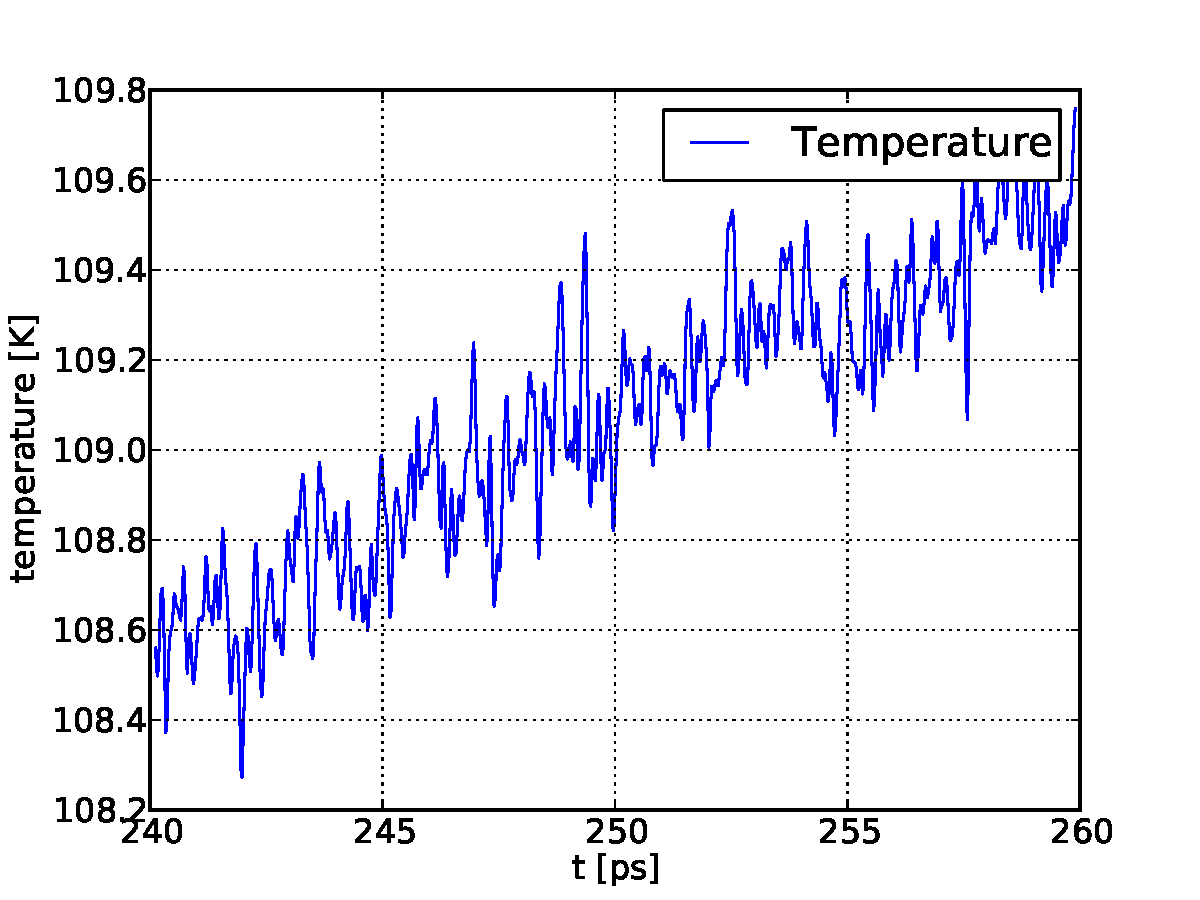
\includegraphics[width=0.45\textwidth]{../analysis/1j-cylinder-force/runs/2013-04-05_201107/1-thermalize/temperature0_90.pdf}
  % flow-profile-02.pdf: 576x432 pixel, 72dpi, 20.32x15.24 cm, bb=0 0 576 432
  \caption{At the end of the simulation, there is still an evident rise in temperature, indicating that we have not yet reached an equilibrium state for the system.}
  \label{fig:increasing-temperature}
\end{figure}


\subsection{Flow profile}

\begin{figure}
  \centering
  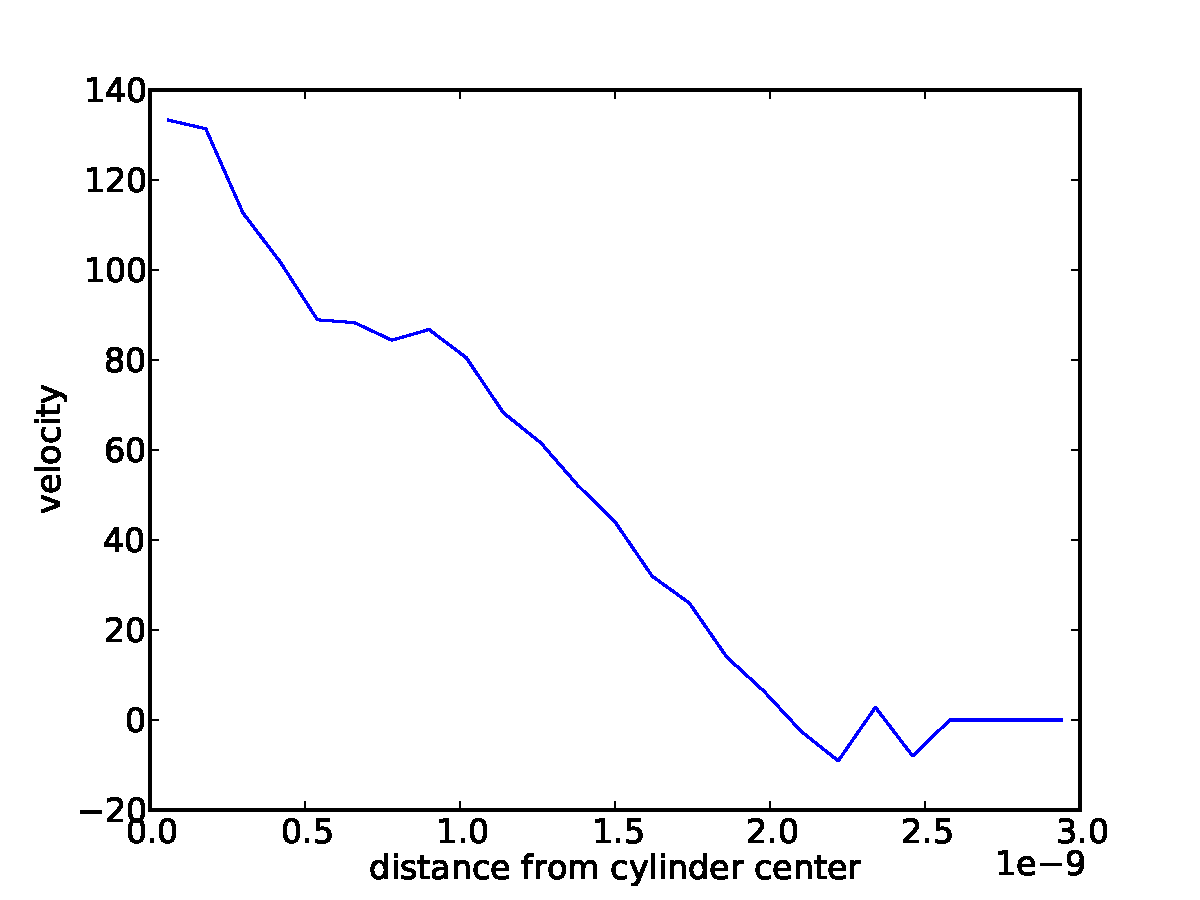
\includegraphics[width=0.45\textwidth]{../analysis/1j-cylinder-force/runs/2013-04-05_201107/flow-profile.pdf}
  % flow-profile-02.pdf: 576x432 pixel, 72dpi, 20.32x15.24 cm, bb=0 0 576 432
  \caption{The flow profile of the system consisting of only one open cylinder. The system was set up with half density inside the cylinder and was exposed to a force in the same direction as the cylinder.}
  \label{fig:flow-profile}
\end{figure}

A plot showing the flow profile is shown in figure \ref{fig:flow-profile}. It is not perfectly parabolic, but the trend is not far from what we could expect. There is more friction along the walls, so the velocity should be higher closer to the middle.

\subsection{Density profile}

\begin{figure}
  \centering
  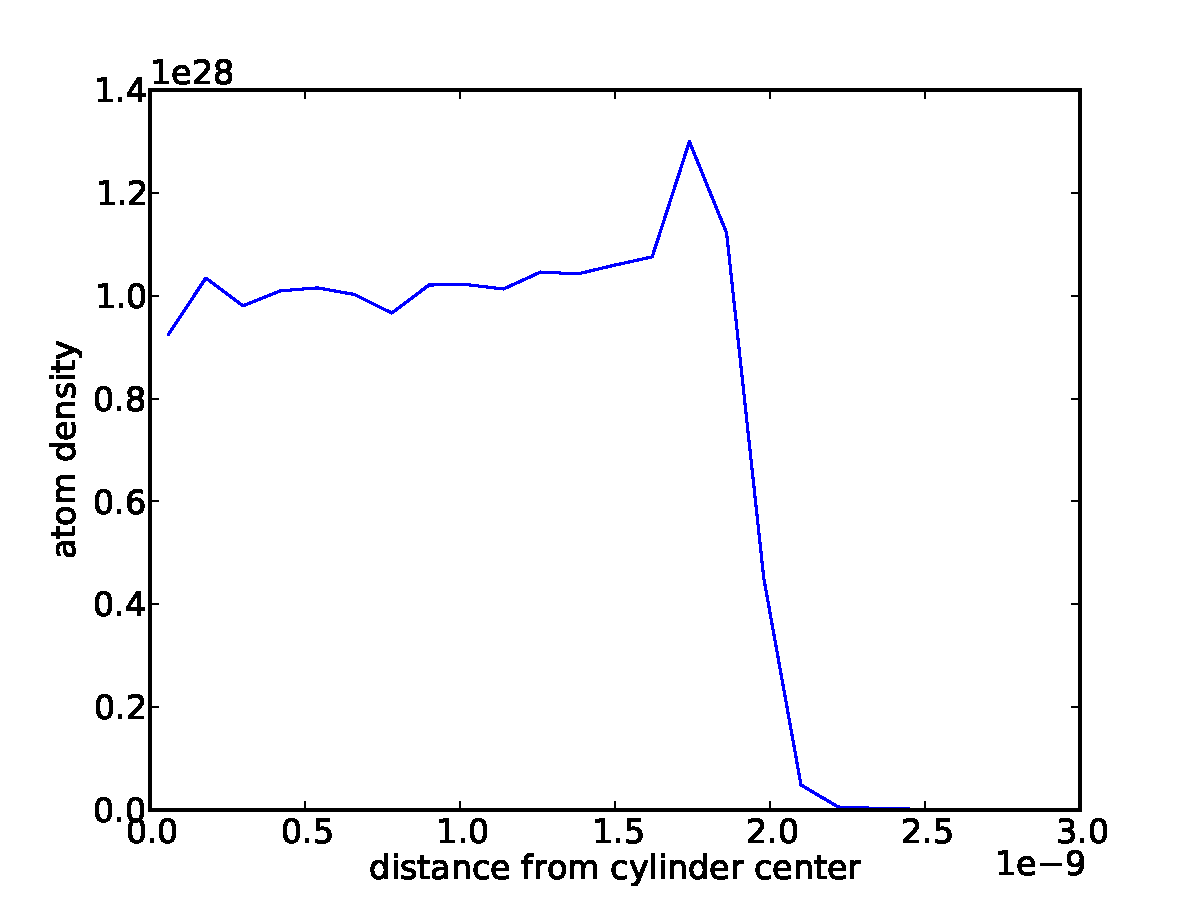
\includegraphics[width=0.45\textwidth]{../analysis/1j-cylinder-force/runs/2013-04-05_201107/atom-density.pdf}
  % atom-density.pdf: 576x432 pixel, 72dpi, 20.32x15.24 cm, bb=0 0 576 432
  \caption{Density profile for the cylinder.}
  \label{fig:density-profile}
\end{figure}

In figure \ref{fig:density-profile} we see a plot showing the density profile of atoms inside the cylinder. We see that the atoms are more located close to the edges of the cylinder. At earlier points in time, the atoms are more localized along the edges, likely because of the attraction to the atoms in the bulk part of the material. After applying the force for some time, the atoms become more localized around the center of the system due to lower ``friction'' from the edges in this area.

\begin{figure}
  \centering
  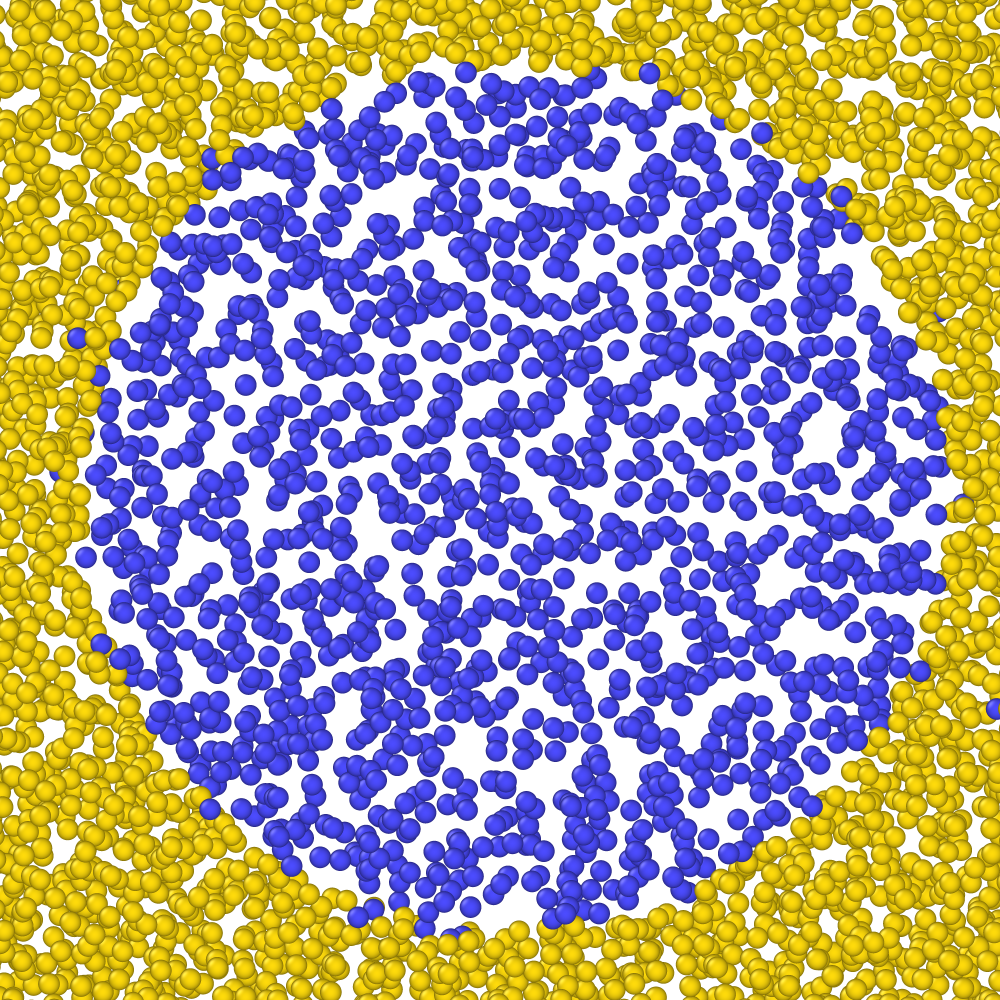
\includegraphics[width=0.30\textwidth]{../analysis/1j-cylinder-force/runs/2013-04-05_201107/density-snapshot.png}
  % density-snapshot.png: 1000x1000 pixel, 99dpi, 25.65x25.65 cm, bb=0 0 727 727
  \caption{Snapshot of the system looking into the cylinder showing that the density is higher along the edges of the cylinder.}
  \label{fig:density-snapshot}
\end{figure}

The density profile is clearly matching the density snapshot shown in figure \ref{fig:density-snapshot}.

\subsection{Displacements in the spherical porous structure}

\begin{figure*}
  \centering
  \begin{subfigure}
    \centering
    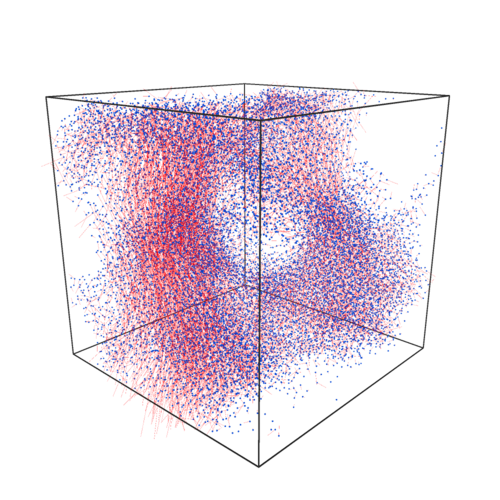
\includegraphics[width=0.23\textwidth]{../analysis/1k-permeability/runs/2013-04-05_201140/frozenpores24/4-way-1.png}
  \end{subfigure}
  \begin{subfigure}
    \centering
    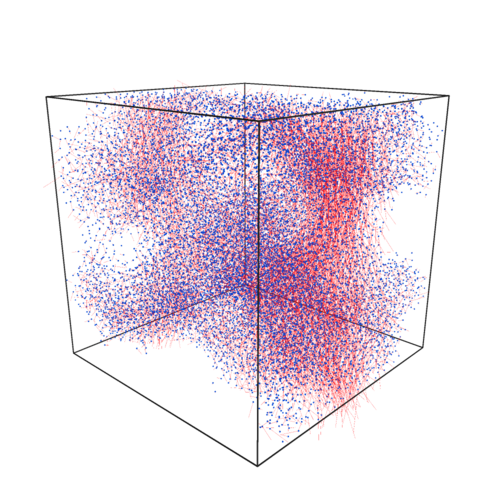
\includegraphics[width=0.23\textwidth]{../analysis/1k-permeability/runs/2013-04-05_201140/frozenpores24/4-way-2.png}
  \end{subfigure}
  \begin{subfigure}
    \centering
    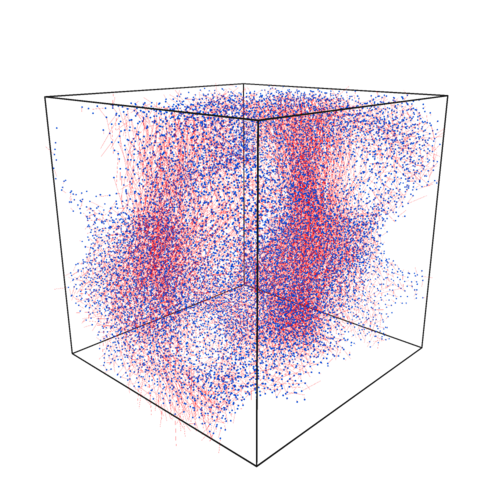
\includegraphics[width=0.23\textwidth]{../analysis/1k-permeability/runs/2013-04-05_201140/frozenpores24/4-way-3.png}
  \end{subfigure}
  \begin{subfigure}
    \centering
    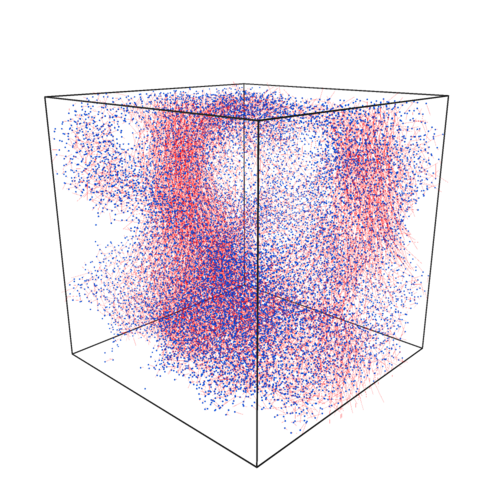
\includegraphics[width=0.23\textwidth]{../analysis/1k-permeability/runs/2013-04-05_201140/frozenpores24/4-way-4.png}
  \end{subfigure}
  % density-snapshot.png: 1000x1000 pixel, 99dpi, 25.65x25.65 cm, bb=0 0 727 727
  \caption{4-way view of the displacements in the spherically nanoporous medium made from 24 frozen spheres (not shown). The displacement vectors are colored red while the atoms are colored blue. It is evident that there are regions with much more flow than others.}
  \label{fig:4-way}
\end{figure*}

\begin{figure}
  \centering
  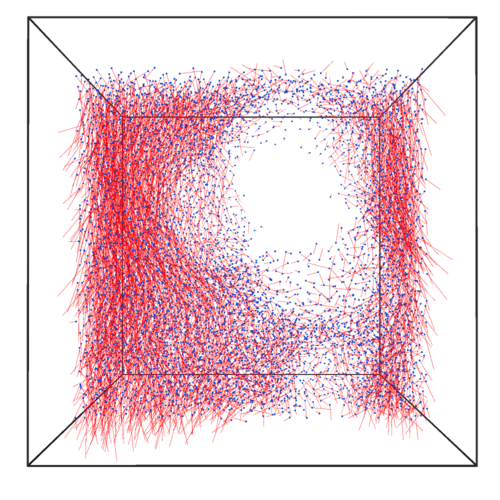
\includegraphics[width=0.45\textwidth]{../analysis/1k-permeability/runs/2013-04-05_201140/frozenpores24/side-view.png}
  % viscosity.pdf: 576x432 pixel, 72dpi, 20.32x15.24 cm, bb=0 0 576 432
  \caption{Displacement vectors calculated for the $1000$ final time steps for the case with 24 frozen spherical pores. Atoms are shown in blue while displacement vectors are colored red.}
  \label{fig:side-view}
\end{figure}

Displacement vectors for the final $1000$ time steps have been calculated for the case with 24 frozen spherical pores and shown graphically in figure \ref{fig:4-way}. We see here that there are regions with much more flow than others (displacement vectors are colored red). The region with most flow has been separated and plotted from a side-view in figure \ref{fig:side-view}.

\subsection{Permeability}
%
\begin{figure}
  \centering
  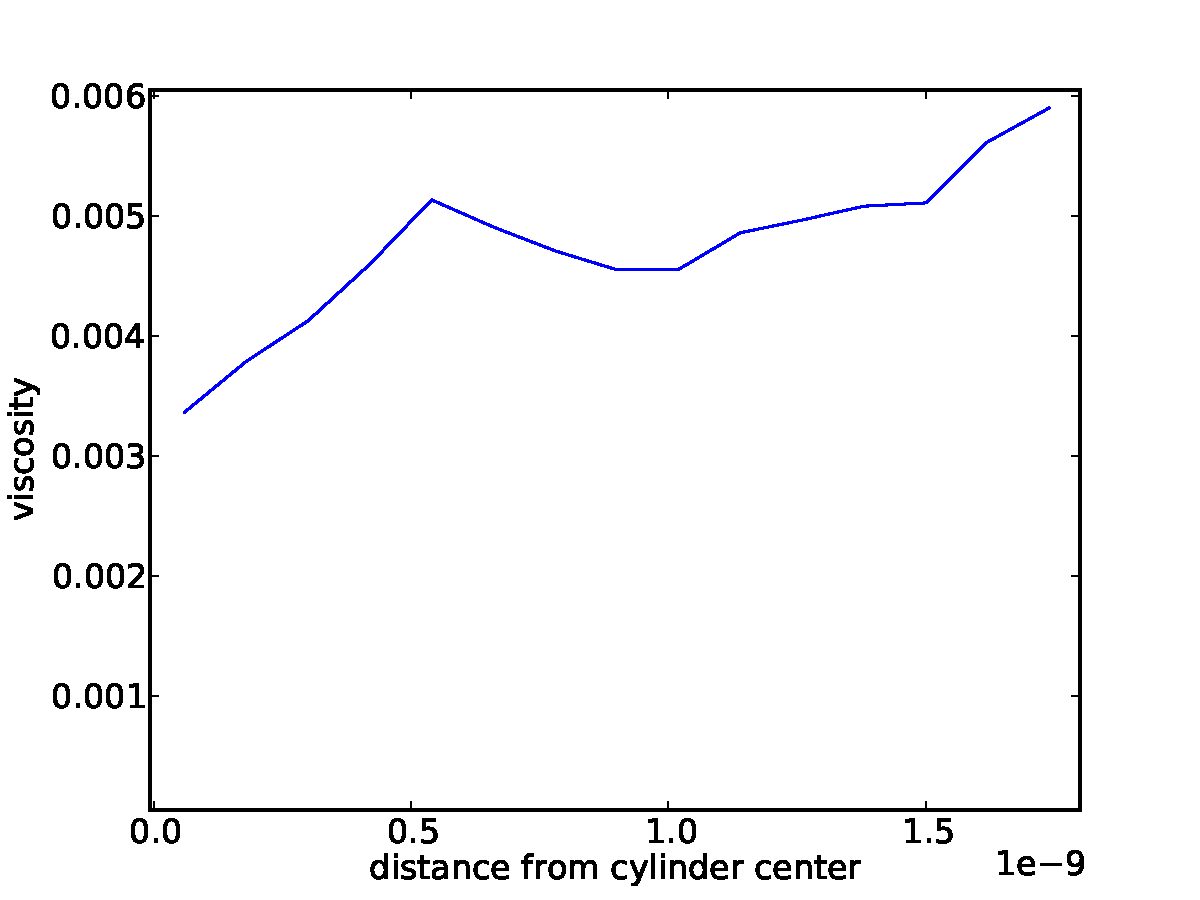
\includegraphics[width=0.45\textwidth]{../analysis/1j-cylinder-force/runs/2013-04-05_201107/viscosity.pdf}
  % viscosity.pdf: 576x432 pixel, 72dpi, 20.32x15.24 cm, bb=0 0 576 432
  \caption{This plot shows the value of $\mu$ which should have been constant. Even though we could have hoped for a viscosity constant throughout the medium, we may estimate a viscosity of about $\mu = 0.005$ by inspection.}
  \label{fig:viscosity-plot}
\end{figure}
%
%
See figure \ref{fig:viscosity-plot} for the plot made by calculating
\begin{equation}
  \mu(r) = \frac{F_{z}(a^2 - r^2)}{4 u(r)}
\end{equation}
%
From this calculation, the viscosity was found to be about
%
\begin{equation}
  \mu = 0.005 \unit{kg/(s\cdot m)}
\end{equation} 
%
for the cylinder.
%
The next needed calculation was the discharge $U$ for different porosities. This is shown in figure \ref{fig:discharges}. In this plot, we've found that only three points are useful for our measurement. The others show systems with either too much or too little flow to give us any good measure of the permeability. Using these three points, we get a linear relation between porosity and discharge.

From Darcy's law, we find the permeability to be
\begin{equation}
  k = \frac{U\mu}{-nF_z}
\end{equation} 
Here we have $nF_z = 78.301 \unit{N/m^{3}}$ and from the discharge plot, we have three values of $U$ that are useful around $U = 50 \unit{m^{3}/ s}$. The incline in this area is $U = 280 \phi$. The permeability is
\begin{equation}
  k = U \cdot 6.39 \cdot 10^{-5} \unit{m \cdot s}
\end{equation} 
Which gives
\begin{equation}
  k =  \phi\cdot 1.79 \cdot 10^{-2} \unit{m^4}
\end{equation} 
I would assume the unit for permeability to be $\unit{m^{2}}$ and not $\unit{m^{4}}$, so something might be wrong with the units in these calculations.

In comparison with the materials listed on \href{http://en.wikipedia.org/wiki/Permeability_\%28earth_sciences\%29}{Wikipedia - Permeability}, the material is as permeable as highly fractured rocks or gravel. I.e. very, very permeable. Given that I've got the wrong units for the permeability, these results should not be trusted too much.
%
\begin{figure}
  \centering
  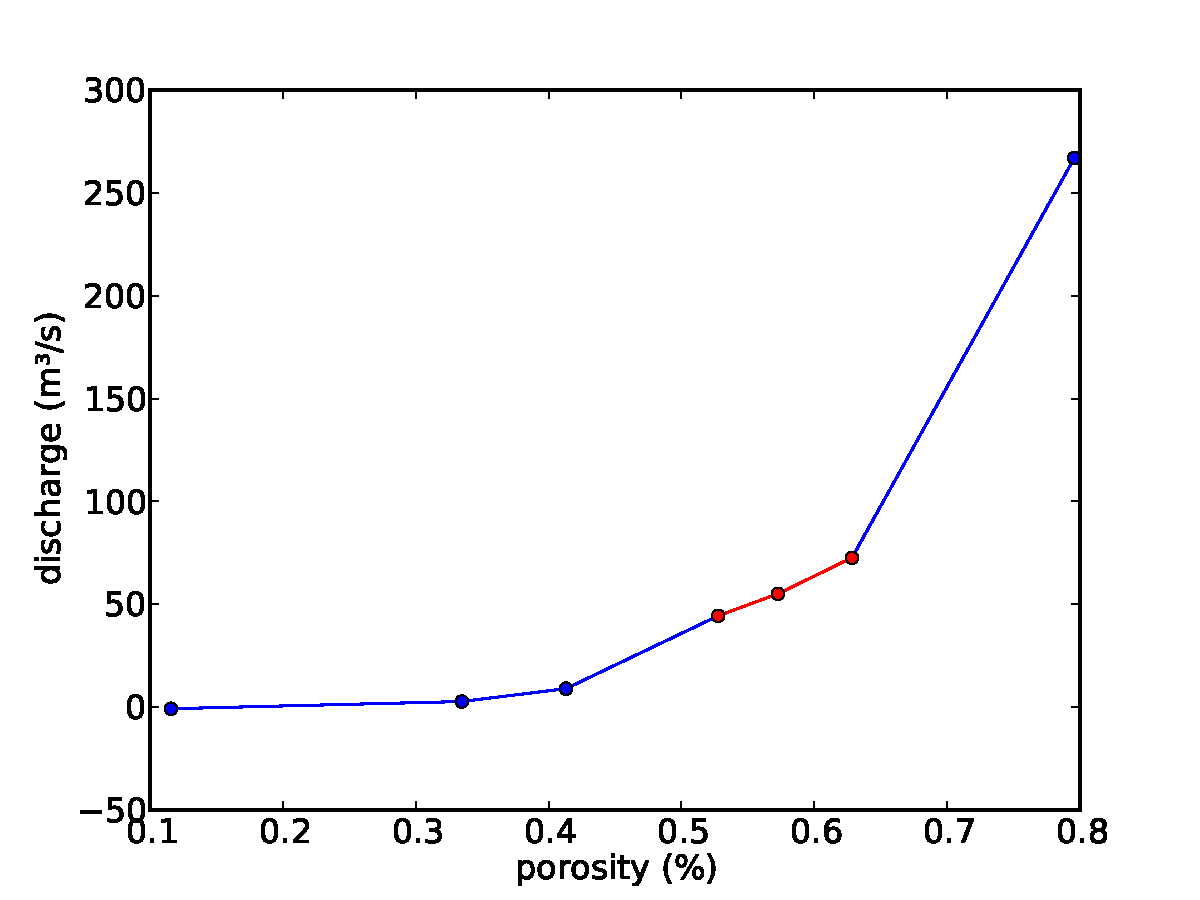
\includegraphics[width=0.45\textwidth]{../analysis/1k-permeability/runs/2013-04-05_201140/discharge.pdf}
  % viscosity.pdf: 576x432 pixel, 72dpi, 20.32x15.24 cm, bb=0 0 576 432
  \caption{Discharge as a function of porosity. The blue points are for systems for which (by observation) there is either too much flow, or no flow at all. These are for 8, 28, 32, and 64 frozen pores, respectively. Only the red points have therefore been taken into consideration when calculating the permeability.}
  \label{fig:discharges}
\end{figure}
%
\appendix

% \section{Conversion to atomic units}


\bibliographystyle{abbrvnat}
\bibliography{references}

\end{document}
